% REMEMBER: You must not plagiarise anything in your report. Be extremely careful.

\documentclass{l4proj}

    
%
% put any additional packages here
%

\begin{document}

%==============================================================================
%% METADATA
\title{This will be the title one day}
\author{Paul E. B. Bekaert}
\date{September 14, 2018}

\maketitle

%==============================================================================
%% ABSTRACT
\begin{abstract}
    Every abstract follows a similar pattern. Motivate; set aims; describe work; explain results.
    \vskip 0.5em
    ``XYZ is bad. This project investigated ABC to determine if it was better. 
    ABC used XXX and YYY to implement ZZZ. This is particularly interesting as XXX and YYY have
    never been used together. It was found that  
    ABC was 20\% better than XYZ, though it caused rabies in half of subjects.''
\end{abstract}

%==============================================================================

% EDUCATION REUSE CONSENT FORM
% If you consent to your project being shown to future students for educational purposes
% then insert your name and the date below to  sign the education use form that appears in the front of the document. 
% You must explicitly give consent if you wish to do so.
% If you sign, your project may be included in the Hall of Fame if it scores particularly highly.
%
% Please note that you are under no obligation to sign 
% this declaration, but doing so would help future students.
%
\def\consentname {Paul E. B. Bekaert} % your full name
\def\consentdate {7 October 2022} % the date you agree
%
\educationalconsent


%==============================================================================
\tableofcontents

%==============================================================================
%% Notes on formatting
%==============================================================================
% The first page, abstract and table of contents are numbered using Roman numerals and are not
% included in the page count. 
%
% From now on pages are numbered
% using Arabic numerals. Therefore, immediately after the first call to \chapter we need the call
% \pagenumbering{arabic} and this should be called once only in the document. 
%
% Do not alter the bibliography style.
%
% The first Chapter should then be on page 1. You are allowed 40 pages for a 40 credit project and 30 pages for a 
% 20 credit report. This includes everything numbered in Arabic numerals (excluding front matter) up
% to but excluding the appendices and bibliography.
%
% You must not alter text size (it is currently 10pt) or alter margins or spacing.
%
%
%==================================================================================================================================
%
% IMPORTANT
% The chapter headings here are **suggestions**. You don't have to follow this model if
% it doesn't fit your project. Every project should have an introduction and conclusion,
% however. 
%
%==================================================================================================================================
\chapter{Introduction}

% reset page numbering. Don't remove this!
\pagenumbering{arabic} 

Why should the reader care about what are you doing and what are you actually doing?

\section{Motivation}

The game of life has often been seen as a toy project. It is idealistic in its representation, as it is fully observable, episodic and deterministic. However, its simple rules give rise to complex structures that are not easy to find. Those structures can be large, and looking for them is unfeasible with the current methods. In general, conventional graph search methods adapted to the task are are used, but they are slow and require large amounts of memory \cite{list_of_search_algorithms}, and as mentioned, they cannot find objects that are too large. There is, as of yet, no efficient way to search for these structures, and the question remains if there is a way to do it.

The concept of using deep learning to find structures in cellular automata has not yet been explored. With the advent and rise of neural networks, previously thought to be impossible problems have been unlocked, either by solving them directly or speeding up existing search algorithms. Since this is a difficult search problem, it stands to reason that solving it will potentially give new insights into how to solve similar problems.

\section{Aims}

In this paper, we will be trying to find interesting structures in the game of life. Our particular interest will be in oscillating objects that move a set amount of space, so-called 'Spaceships'. The main goal will be to test and see if neural networks can speed up the search, and how different deep learning techniques fare against each other and other conventional search methods. The expectation is that the network will greatly decrease the time it takes to find novel structures, or recognise structures that are classified as spaceships.


%==================================================================================================================================
\chapter{Background}
What did other people do, and how is it relevant to what you want to do?
\section{The game of life}
% ========

\subsection{Rules}

"The Game of Life" is a zero-player game invented by John Conway in 1969? which describes a cellular automata (CA) with a set of rules. The board is made out of a grid $n\times m$ is created, with each square being a cell. A cell is either dead or alive, represented as a $1$ or a $0$ respectively. The rules of the game can be defined in different ways, but the one John Conway proposed is the most well known. The neighbourhood of the cell is defined as Moore's neighbourhood, which is the 8 cells adjacent to the cell, diagonally and orthogonally. It can also be thought of as a $3\times 3$ matrix where the subject cell is placed in the middle. The number of neighbours the cell has is the number of cells alive that are present in the cell's Moore neighbourhood, $n$. We can then define the rules of the CA described in Life:

\begin{itemize}
    \item A dead cell turns into a living cell if $n \geq 3$
    \item A dead cell stays dead if $n < 3$
    \item A living cell stays alive if $n = 2$ or $n = 3$
    \item A living cell dies if $n < 2$, due to under-population
    \item A living cell dies if $n > 3$, due to overcrowding
\end{itemize}

A state at $t+1$ is entirely dependant on the current state at $t$ and is calculated using the rules above.

\begin{figure}[h]

\begin{subfigure}{0.5\textwidth}
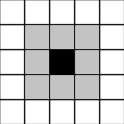
\includegraphics[width=0.9\linewidth, height=6cm]{dissertation/images/moores_law.png} 
\caption{Moore's Neighbourhood}
\label{fig:subim1}
\end{subfigure}
\begin{subfigure}{0.5\textwidth}
\includegraphics[width=0.9\linewidth, height=6cm]{dissertation/images/boxplot_finger_distance.pdf}
\caption{Another one}
\label{fig:subim2}
\end{subfigure}

\caption{Examples of Moore's neighbourhood}
\label{fig:image2}
\end{figure}

\subsection{Still lifes}

A still life is a structure that does not move or change shape from generation to generation. They remain static, unless outside cells interact with it. Still lifes are by far the most known structures in the GoL, and they are easy to find, as they have the same shape for $t$ and $t+1$. Here are some examples of still lifes:

\subsection{Oscillators}

These are structures that change shape, but return to the same state every $p$ generations. They are a little harder to detect, as it is impossible to know how many generations it will take for the structure to repeat. An oscillator will stay in the same position after it has oscillated, and will keep oscillating as long as it is undisturbed by other cells and the program keeps running. Here are some examples of oscillators:

\subsection{Spaceships}

Spaceships are the main focus of this paper, and are the hardest structures to detect. They are similar to oscillators in that they repeat their state every $p$ generations. However, they also move a certain distance since their last oscillation. If the state space they are in is unbounded, then they will move forever without changing direction.

The speed of a spaceship is determined in terms of the speed of light of GoL, $c$. This $c$ is defined as 1 cell per second, as it is theoretically the quickest information could hope to propagate given the rules of Life. The ship can move diagonally, orthogonally, or knightwise, which is when a ship moves in an oblique direction. A spaceship with a period $p$, which is moving $n$ cells in a particular direction is said to have a speed $nc/p$. A ship moving $n = 2$ cells left and with a period $p = 5$ will have a speed of $2c/5$. For a ship moving knightwise $n$ cells either left or right, and $m$ cells either up or down, will have a speed denoted as $(m, n)c/p$. These speeds can be simplified, for example a spaceship moving at speed $2c/4$ can be written as $c/2$.

A further way to classify spaceships is by their type. 
% should you explain this?

Examples of spaceships:


% ========
\section{Existing Search Methods}

\subsection{Brute Force Search of Spaceships}

Brute force search for the game of life is wildly inefficient. The problem, as with most brute force algorithms, is that there are too many possibilities to check, and therefore a comprehensive search is impossible with current processing power. In a given $n \times m$ grid, there are $2^{n \times m}$ possible combinations. For example, a glider, which takes at least a $3x3$ grid to be represented, would be found by searching $2^{9}$ grids. Brute force becomes unfeasible after approximately $n > 6, m > 6$. These algorithms tend not to have much use, but have found a comprehensive list of all still-lives, oscillators, and spaceships within a small rectangle.
 
\subsection{Graph Search}

One notable paper is "Searching for Spaceships" \cite{searching_for_spaceships}, which uses an algorithm "gfind", using a mix of breadth first search and depth first iterative deepening. The search takes place row-by-row, and uses a pre-calculated hash table of cell configurations to remove impossible rows from the search, narrowing down the graph. This method only works for small periods, as larger ones run out of memory quite quickly. It also only finds orthogonal spaceships, and they must be symmetrical along one of its axis. It was used to find some common spaceships, and did improve on speed, but did have its limitations.

Another well known algorithm to find spaceships or oscillators is "lifesrc" created by David Bell, uses a depth first backtracking search. The grid is first set up with a few 'known' cells, set by the user. The rest of the cells are classed as 'unknown'. When the algorithm starts running, a decision is made on whether a cell should be alive or not, and the program will check forward and backward if there are any oscillating patterns of period $p$ set by the user. If nothing is found, the search continues, using the decided cell. If it is found later on that a cell placement in a particular cell is impossible, or that there are no oscillators in a particular configuration, then the algorithm will backtrack to the latest cell it decided on randomly. This is essentially a depth first search, however it discards certain sub-trees by eliminating ones that do not follow the Life rules (for example, checking if every cell is alive would be redundant, since there would be no oscillators in that configuration). This algorithm is efficient and was used to find a lot of the different life spaceships or oscillators.

\section{Deep Learning with the GoL in General}

There are a few research papers written on neural networks and the game of life,
paper about forward learning GoL
paper about population density

Apart from research done, there are many hobbyists working on combining deep learning with GoL. One of them is James McGuigan, who trained a neural network to learn the game of life after one iteration. He also worked on reversing the game of life, trying to find a previous configuration using a current board state. Another notable use of deep learning and the game of life is by NeatAI, who used genetic algorithms in the game of life \cite{neatai_gol}. He used a $c$ function that calculates the overall 'complexity' of the current structures in the grid. For example, a grid with random cells is not very interesting, but one that has a couple of gliders and oscillators with high periods may be of more interest. To design his $c£$ function, he took inspiration from a paper by \cite{algorithmic_specified_complexity}, which describes a process of encoding interesting objects in the game of life. It uses features of an object such as shift, repeating period, intersection between 2 or more objects, to define the properties of such an object, These properties are then bit-encoded to form a number that specifies the complexity of the object. To find the complexity of a particular state on a board, the sum of the object complexities is taken.

NeatAI took this $c$ function and applied it to a neural network which determined whether or not a cell should be alive given the input parameters $x$, $y$, population density, and bias. He then used genetic neural networks to improve his model to maximize the $c$ function. The net improved by making optimal start configurations for the model to evolve into. This is an interesting concept, as if the $c$ function were to be changed to be maximised by how far a pattern has reached from the origin, it could potentially be used to find new spaceships for example.

%==================================================================================================================================

\chapter{Analysis/Requirements}
What is the problem that you want to solve, and how did you arrive at it?
\section{Guidance}
Make it clear how you derived the constrained form of your problem via a clear and logical process. 

%==================================================================================================================================
\chapter{Design}
How is this problem to be approached, without reference to specific implementation details? 
\section{Guidance}
Design should cover the abstract design in such a way that someone else might be able to do what you did, but with a different language or library or tool.

%==================================================================================================================================
\chapter{Implementation}
What did you do to implement this idea, and what technical achievements did you make?
\section{Guidance}
You can't talk about everything. Cover the high level first, then cover important, relevant or impressive details.



\section{General points}

These points apply to the whole dissertation, not just this chapter.



\subsection{Figures}
\emph{Always} refer to figures included, like Figure \ref{fig:relu}, in the body of the text. Include full, explanatory captions and make sure the figures look good on the page.
You may include multiple figures in one float, as in Figure \ref{fig:synthetic}, using \texttt{subcaption}, which is enabled in the template.



% Figures are important. Use them well.
\begin{figure}
    \centering
    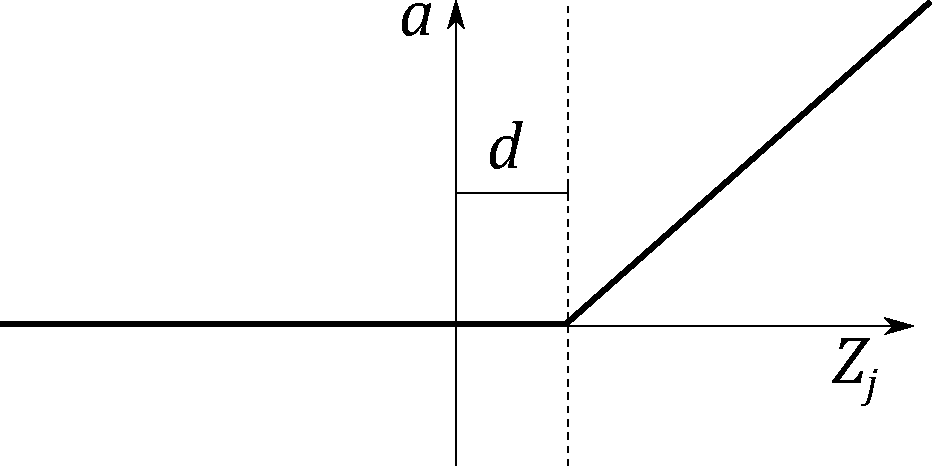
\includegraphics[width=0.5\linewidth]{images/relu.pdf}    

    \caption{In figure captions, explain what the reader is looking at: ``A schematic of the rectifying linear unit, where $a$ is the output amplitude,
    $d$ is a configurable dead-zone, and $Z_j$ is the input signal'', as well as why the reader is looking at this: 
    ``It is notable that there is no activation \emph{at all} below 0, which explains our initial results.'' 
    \textbf{Use vector image formats (.pdf) where possible}. Size figures appropriately, and do not make them over-large or too small to read.
    }

    % use the notation fig:name to cross reference a figure
    \label{fig:relu} 
\end{figure}


\begin{figure}
    \centering
    \begin{subfigure}[b]{0.45\textwidth}
        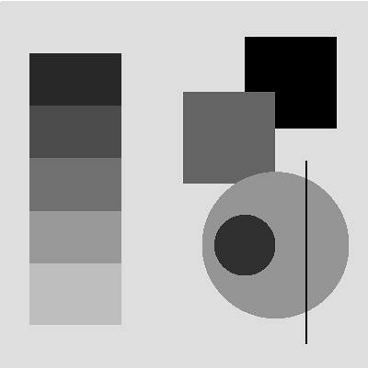
\includegraphics[width=\textwidth]{images/synthetic.png}
        \caption{Synthetic image, black on white.}
        \label{fig:syn1}
    \end{subfigure}
    ~ %add desired spacing between images, e. g. ~, \quad, \qquad, \hfill etc. 
      %(or a blank line to force the subfigure onto a new line)
    \begin{subfigure}[b]{0.45\textwidth}
        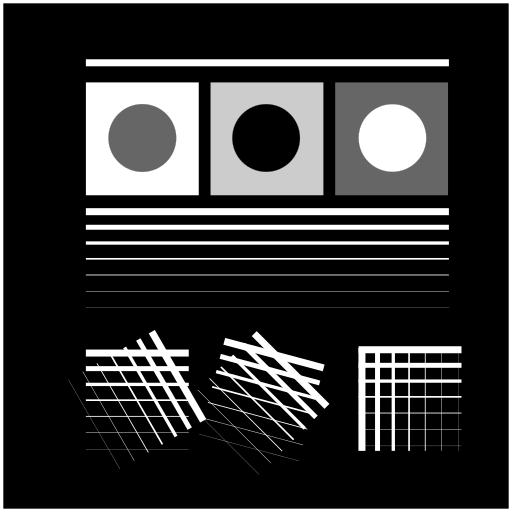
\includegraphics[width=\textwidth]{images/synthetic_2.png}
        \caption{Synthetic image, white on black.}
        \label{fig:syn2}
    \end{subfigure}
    ~ %add desired spacing between images, e. g. ~, \quad, \qquad, \hfill etc. 
    %(or a blank line to force the subfigure onto a new line)    
    \caption{Synthetic test images for edge detection algorithms. \subref{fig:syn1} shows various gray levels that require an adaptive algorithm. \subref{fig:syn2}
    shows more challenging edge detection tests that have crossing lines. Fusing these into full segments typically requires algorithms like the Hough transform.
    This is an example of using subfigures, with \texttt{subref}s in the caption.
    }\label{fig:synthetic}
\end{figure}

\clearpage

\subsection{Equations}

Equations should be typeset correctly and precisely. Make sure you get parenthesis sizing correct, and punctuate equations correctly 
(the comma is important and goes \textit{inside} the equation block). Explain any symbols used clearly if not defined earlier. 

For example, we might define:
\begin{equation}
    \hat{f}(\xi) = \frac{1}{2}\left[ \int_{-\infty}^{\infty} f(x) e^{2\pi i x \xi} \right],
\end{equation}    
where $\hat{f}(\xi)$ is the Fourier transform of the time domain signal $f(x)$.

\subsection{Algorithms}
Algorithms can be set using \texttt{algorithm2e}, as in Algorithm \ref{alg:metropolis}.

% NOTE: line ends are denoted by \; in algorithm2e
\begin{algorithm}
    \DontPrintSemicolon
    \KwData{$f_X(x)$, a probability density function returing the density at $x$.\; $\sigma$ a standard deviation specifying the spread of the proposal distribution.\;
    $x_0$, an initial starting condition.}
    \KwResult{$s=[x_1, x_2, \dots, x_n]$, $n$ samples approximately drawn from a distribution with PDF $f_X(x)$.}
    \Begin{
        $s \longleftarrow []$\;
        $p \longleftarrow f_X(x)$\;
        $i \longleftarrow 0$\;
        \While{$i < n$}
        {
            $x^\prime \longleftarrow \mathcal{N}(x, \sigma^2)$\;
            $p^\prime \longleftarrow f_X(x^\prime)$\;
            $a \longleftarrow \frac{p^\prime}{p}$\;
            $r \longleftarrow U(0,1)$\;
            \If{$r<a$}
            {
                $x \longleftarrow x^\prime$\;
                $p \longleftarrow f_X(x)$\;
                $i \longleftarrow i+1$\;
                append $x$ to $s$\;
            }
        }
    }
    
\caption{The Metropolis-Hastings MCMC algorithm for drawing samples from arbitrary probability distributions, 
specialised for normal proposal distributions $q(x^\prime|x) = \mathcal{N}(x, \sigma^2)$. The symmetry of the normal distribution means the acceptance rule takes the simplified form.}\label{alg:metropolis}
\end{algorithm}

\subsection{Tables}

If you need to include tables, like Table \ref{tab:operators}, use a tool like https://www.tablesgenerator.com/ to generate the table as it is
extremely tedious otherwise. 

\begin{table}[]
    \caption{The standard table of operators in Python, along with their functional equivalents from the \texttt{operator} package. Note that table
    captions go above the table, not below. Do not add additional rules/lines to tables. }\label{tab:operators}
    %\tt 
    \rowcolors{2}{}{gray!3}
    \begin{tabular}{@{}lll@{}}
    %\toprule
    \textbf{Operation}    & \textbf{Syntax}                & \textbf{Function}                            \\ %\midrule % optional rule for header
    Addition              & \texttt{a + b}                          & \texttt{add(a, b)}                                    \\
    Concatenation         & \texttt{seq1 + seq2}                    & \texttt{concat(seq1, seq2)}                           \\
    Containment Test      & \texttt{obj in seq}                     & \texttt{contains(seq, obj)}                           \\
    Division              & \texttt{a / b}                          & \texttt{div(a, b) }  \\
    Division              & \texttt{a / b}                          & \texttt{truediv(a, b) } \\
    Division              & \texttt{a // b}                         & \texttt{floordiv(a, b)}                               \\
    Bitwise And           & \texttt{a \& b}                         & \texttt{and\_(a, b)}                                  \\
    Bitwise Exclusive Or  & \texttt{a \textasciicircum b}           & \texttt{xor(a, b)}                                    \\
    Bitwise Inversion     & \texttt{$\sim$a}                        & \texttt{invert(a)}                                    \\
    Bitwise Or            & \texttt{a | b}                          & \texttt{or\_(a, b)}                                   \\
    Exponentiation        & \texttt{a ** b}                         & \texttt{pow(a, b)}                                    \\
    Identity              & \texttt{a is b}                         & \texttt{is\_(a, b)}                                   \\
    Identity              & \texttt{a is not b}                     & \texttt{is\_not(a, b)}                                \\
    Indexed Assignment    & \texttt{obj{[}k{]} = v}                 & \texttt{setitem(obj, k, v)}                           \\
    Indexed Deletion      & \texttt{del obj{[}k{]}}                 & \texttt{delitem(obj, k)}                              \\
    Indexing              & \texttt{obj{[}k{]}}                     & \texttt{getitem(obj, k)}                              \\
    Left Shift            & \texttt{a \textless{}\textless b}       & \texttt{lshift(a, b)}                                 \\
    Modulo                & \texttt{a \% b}                         & \texttt{mod(a, b)}                                    \\
    Multiplication        & \texttt{a * b}                          & \texttt{mul(a, b)}                                    \\
    Negation (Arithmetic) & \texttt{- a}                            & \texttt{neg(a)}                                       \\
    Negation (Logical)    & \texttt{not a}                          & \texttt{not\_(a)}                                     \\
    Positive              & \texttt{+ a}                            & \texttt{pos(a)}                                       \\
    Right Shift           & \texttt{a \textgreater{}\textgreater b} & \texttt{rshift(a, b)}                                 \\
    Sequence Repetition   & \texttt{seq * i}                        & \texttt{repeat(seq, i)}                               \\
    Slice Assignment      & \texttt{seq{[}i:j{]} = values}          & \texttt{setitem(seq, slice(i, j), values)}            \\
    Slice Deletion        & \texttt{del seq{[}i:j{]}}               & \texttt{delitem(seq, slice(i, j))}                    \\
    Slicing               & \texttt{seq{[}i:j{]}}                   & \texttt{getitem(seq, slice(i, j))}                    \\
    String Formatting     & \texttt{s \% obj}                       & \texttt{mod(s, obj)}                                  \\
    Subtraction           & \texttt{a - b}                          & \texttt{sub(a, b)}                                    \\
    Truth Test            & \texttt{obj}                            & \texttt{truth(obj)}                                   \\
    Ordering              & \texttt{a \textless b}                  & \texttt{lt(a, b)}                                     \\
    Ordering              & \texttt{a \textless{}= b}               & \texttt{le(a, b)}                                     \\
    % \bottomrule
    \end{tabular}
    \end{table}
\subsection{Code}

Avoid putting large blocks of code in the report (more than a page in one block, for example). Use syntax highlighting if possible, as in Listing \ref{lst:callahan}.

\begin{lstlisting}[language=python, float, caption={The algorithm for packing the $3\times 3$ outer-totalistic binary CA successor rule into a 
    $16\times 16\times 16\times 16$ 4 bit lookup table, running an equivalent, notionally 16-state $2\times 2$ CA.}, label=lst:callahan]
    def create_callahan_table(rule="b3s23"):
        """Generate the lookup table for the cells."""        
        s_table = np.zeros((16, 16, 16, 16), dtype=np.uint8)
        birth, survive = parse_rule(rule)

        # generate all 16 bit strings
        for iv in range(65536):
            bv = [(iv >> z) & 1 for z in range(16)]
            a, b, c, d, e, f, g, h, i, j, k, l, m, n, o, p = bv

            # compute next state of the inner 2x2
            nw = apply_rule(f, a, b, c, e, g, i, j, k)
            ne = apply_rule(g, b, c, d, f, h, j, k, l)
            sw = apply_rule(j, e, f, g, i, k, m, n, o)
            se = apply_rule(k, f, g, h, j, l, n, o, p)

            # compute the index of this 4x4
            nw_code = a | (b << 1) | (e << 2) | (f << 3)
            ne_code = c | (d << 1) | (g << 2) | (h << 3)
            sw_code = i | (j << 1) | (m << 2) | (n << 3)
            se_code = k | (l << 1) | (o << 2) | (p << 3)

            # compute the state for the 2x2
            next_code = nw | (ne << 1) | (sw << 2) | (se << 3)

            # get the 4x4 index, and write into the table
            s_table[nw_code, ne_code, sw_code, se_code] = next_code

        return s_table

\end{lstlisting}

%==================================================================================================================================
\chapter{Evaluation} 
How good is your solution? How well did you solve the general problem, and what evidence do you have to support that?

\section{Guidance}
\begin{itemize}
    \item
        Ask specific questions that address the general problem.
    \item
        Answer them with precise evidence (graphs, numbers, statistical
        analysis, qualitative analysis).
    \item
        Be fair and be scientific.
    \item
        The key thing is to show that you know how to evaluate your work, not
        that your work is the most amazing product ever.
\end{itemize}

\section{Evidence}
Make sure you present your evidence well. Use appropriate visualisations, reporting techniques and statistical analysis, as appropriate.

If you visualise, follow the basic rules, as illustrated in Figure \ref{fig:boxplot}:
\begin{itemize}
\item Label everything correctly (axis, title, units).
\item Caption thoroughly.
\item Reference in text.
\item \textbf{Include appropriate display of uncertainty (e.g. error bars, Box plot)}
\item Minimize clutter.
\end{itemize}

See the file \texttt{guide\_to\_visualising.pdf} for further information and guidance.

\begin{figure}
    \centering
    \includegraphics[width=1.0\linewidth]{images/boxplot_finger_distance.pdf}    

    \caption{Average number of fingers detected by the touch sensor at different heights above the surface, averaged over all gestures. Dashed lines indicate
    the true number of fingers present. The Box plots include bootstrapped uncertainty notches for the median. It is clear that the device is biased toward 
    undercounting fingers, particularly at higher $z$ distances.
    }

    % use the notation fig:name to cross reference a figure
    \label{fig:boxplot} 
\end{figure}


%==================================================================================================================================
\chapter{Conclusion}    
Summarise the whole project for a lazy reader who didn't read the rest (e.g. a prize-awarding committee).
\section{Guidance}
\begin{itemize}
    \item
        Summarise briefly and fairly.
    \item
        You should be addressing the general problem you introduced in the
        Introduction.        
    \item
        Include summary of concrete results (``the new compiler ran 2x
        faster'')
    \item
        Indicate what future work could be done, but remember: \textbf{you
        won't get credit for things you haven't done}.
\end{itemize}

%==================================================================================================================================
%
% 
%==================================================================================================================================
%  APPENDICES  

\begin{appendices}

\chapter{Appendices}

Typical inclusions in the appendices are:

\begin{itemize}
\item
  Copies of ethics approvals (required if obtained)
\item
  Copies of questionnaires etc. used to gather data from subjects.
\item
  Extensive tables or figures that are too bulky to fit in the main body of
  the report, particularly ones that are repetitive and summarised in the body.

\item Outline of the source code (e.g. directory structure), or other architecture documentation like class diagrams.

\item User manuals, and any guides to starting/running the software.

\end{itemize}

\textbf{Don't include your source code in the appendices}. It will be
submitted separately.

\end{appendices}

%==================================================================================================================================
%   BIBLIOGRAPHY   

% The bibliography style is abbrvnat
% The bibliography always appears last, after the appendices.

\bibliographystyle{abbrvnat}

\bibliography{l4proj}

\end{document}
